\documentclass[../main.tex]{subfiles}

% ======================== Document: Results ======================== %

\begin{document}
\section{Results}
\label{sec:results}

\subsection{Patent applications}

Table \ref{tab:dd_twfe_patents} presents results the estimation of Equation \ref{eq:dd_model} using patent applications as the explained variable with the province-quarter data. Specification (1) includes a baseline result with no control variables. Specification (2) includes economic controls included to account for factors which may affect the comparability of the treatment and control groups regarding firm activity and overall economic trends which vary across time and provinces. The number of foreign parties in all the province's patent applications is also included, to control for effects that foreign interested parties (particularly U.S.) can have as strategic actors for patent applications. Specification (3) includes additional controls. These are included in the case that the previous controls did not adequately account for differences in trends due to reasons other than economy, or that economic activity is not well captured by standard variables in Specification (2). 

The DD estimate for the causal effect of the AITC intervention is the coefficient on Treatment \texttimes Post, showing that the intervention led to an -6.1\% to +2.3\% change in Albertan patent applications. However, the effect is not statistically distinguishable from zero. Standard errors for this coefficient on all three specifications are small compared to those of the controls, showing that $\hat{\beta}$ is estimated with a fairly good level of precision. This implies that it is the small magnitude of $\hat{\beta}$ which drives the low $p$-value of the hypothesis test, leading to the preliminary conclusion that the AITC intervention had no effect on innovation in the studied period. 

\begin{table}[h]
    \centering
    \label{tab:dd_twfe_patents}
\begin{threeparttable}
    \caption{Difference-in-differences specifications for quarterly patent applications}
    
\begin{tabular}[t]{lccc}
\toprule
  & (1) & (2) & (3)\\
\midrule
Treatment x Post & \num{-0.093}* & \num{0.001} & \num{-0.011}\\
\textbf{} & \textbf{(\num{0.042})} & \textbf{(\num{0.066})} & \textbf{(\num{0.076})}\\
Ln Full-time employment &  & \num{0.756} & \num{1.032}\\
 &  & (\num{0.644}) & (\num{0.646})\\
Ln Median wage &  & \num{1.235}** & \num{1.107}**\\
 &  & (\num{0.387}) & (\num{0.445})\\
CPI &  & \num{-0.015}** & \num{-0.007}\\
 &  & (\num{0.005}) & (\num{0.008})\\
Ln +1 Business insolvencies &  & \num{-0.065}** & \num{-0.051}*\\
 &  & (\num{0.027}) & (\num{0.023})\\
Ln Intl. exports &  & \num{-0.081} & \num{-0.079}\\
 &  & (\num{0.097}) & (\num{0.125})\\
Ln Intl. imports &  & \num{0.016} & \num{0.022}\\
 &  & (\num{0.126}) & (\num{0.127})\\
Ln Retail sales &  & \num{-0.279} & \num{0.094}\\
 &  & (\num{0.421}) & (\num{0.492})\\
Ln Wholesale sales &  & \num{-0.150} & \num{-0.229}\\
 &  & (\num{0.156}) & (\num{0.139})\\
Ln Manufacturing sales &  & \num{0.275} & \num{0.210}\\
 &  & (\num{0.153}) & (\num{0.146})\\
Ln +1 Foreign patent parties &  & \num{0.141}*** & \num{0.135}***\\
 &  & (\num{0.016}) & (\num{0.016})\\
Ln International travellers &  &  & \num{-0.129}***\\
 &  &  & (\num{0.034})\\
Ln Arriving vehicles &  &  & \num{0.007}\\
 &  &  & (\num{0.004})\\
Ln Electric power generation &  &  & \num{0.078}\\
 &  &  & (\num{0.115})\\
Ln Average actual hours &  &  & \num{0.109}\\
 &  &  & (\num{0.277})\\
New housing price index &  &  & \num{-0.003}\\
 &  &  & (\num{0.002})\\
Ln Food services receipts &  &  & \num{-0.080}\\
 &  &  & (\num{0.201})\\
Ln Average job tenure &  &  & \num{-0.424}\\
 &  &  & (\num{0.373})\\
\midrule
Explained variable &  & $\ln(\text{Patents}+1)$ & \\
$N$ & \num{656} & \num{656} & \num{656}\\
Adj. $R^2$ & \num{0.975} & \num{0.980} & \num{0.980}\\
Adj. within $R^2$ & \num{0.002} & \num{0.205} & \num{0.210}\\
RMSE & \num{0.206} & \num{0.182} & \num{0.180}\\
\bottomrule
\end{tabular}
}
    \begin{tablenotes}
        \small
        \item \textit{Notes}: Clustered standard errors at the province and quarter level shown in parentheses. All specifications include fixed effects for provinces and quarters. ***$p<0.01$, **$p<0.05$, *$p<0.1$.
    \end{tablenotes}
\end{threeparttable}
\end{table}

I display the results of the event study regressions in Figure \ref{fig:event_study_patents}. I estimated Equation \ref{eq:event_study} with the same controls as the specifications in Table \ref{tab:dd_twfe_patents}, resulting in panels (1) through (3) plotted in Figure \ref{fig:event_study_patents}. Most importantly these results show that, when controlling for time and province-varying factors, there is not a statistically significant difference between Albertan and control provinces' patent applications before the AITC intervention. This supports the key identifying assumption of the DD design, that the control and treatment groups would have followed the same trend in the absence of the intervention. The baseline model, which does not consider any controls, shows several pre-policy periods where the treatment and control groups diverge, underscoring the importance of including controls in the model. In 2015Q4, there is a positive and significant deviation from the pre-policy trend. 

\begin{figure}[h]
    \centering
    \caption{Event study of the AITC intervention on quarterly patent applications}
    \label{fig:event_study_patents}
    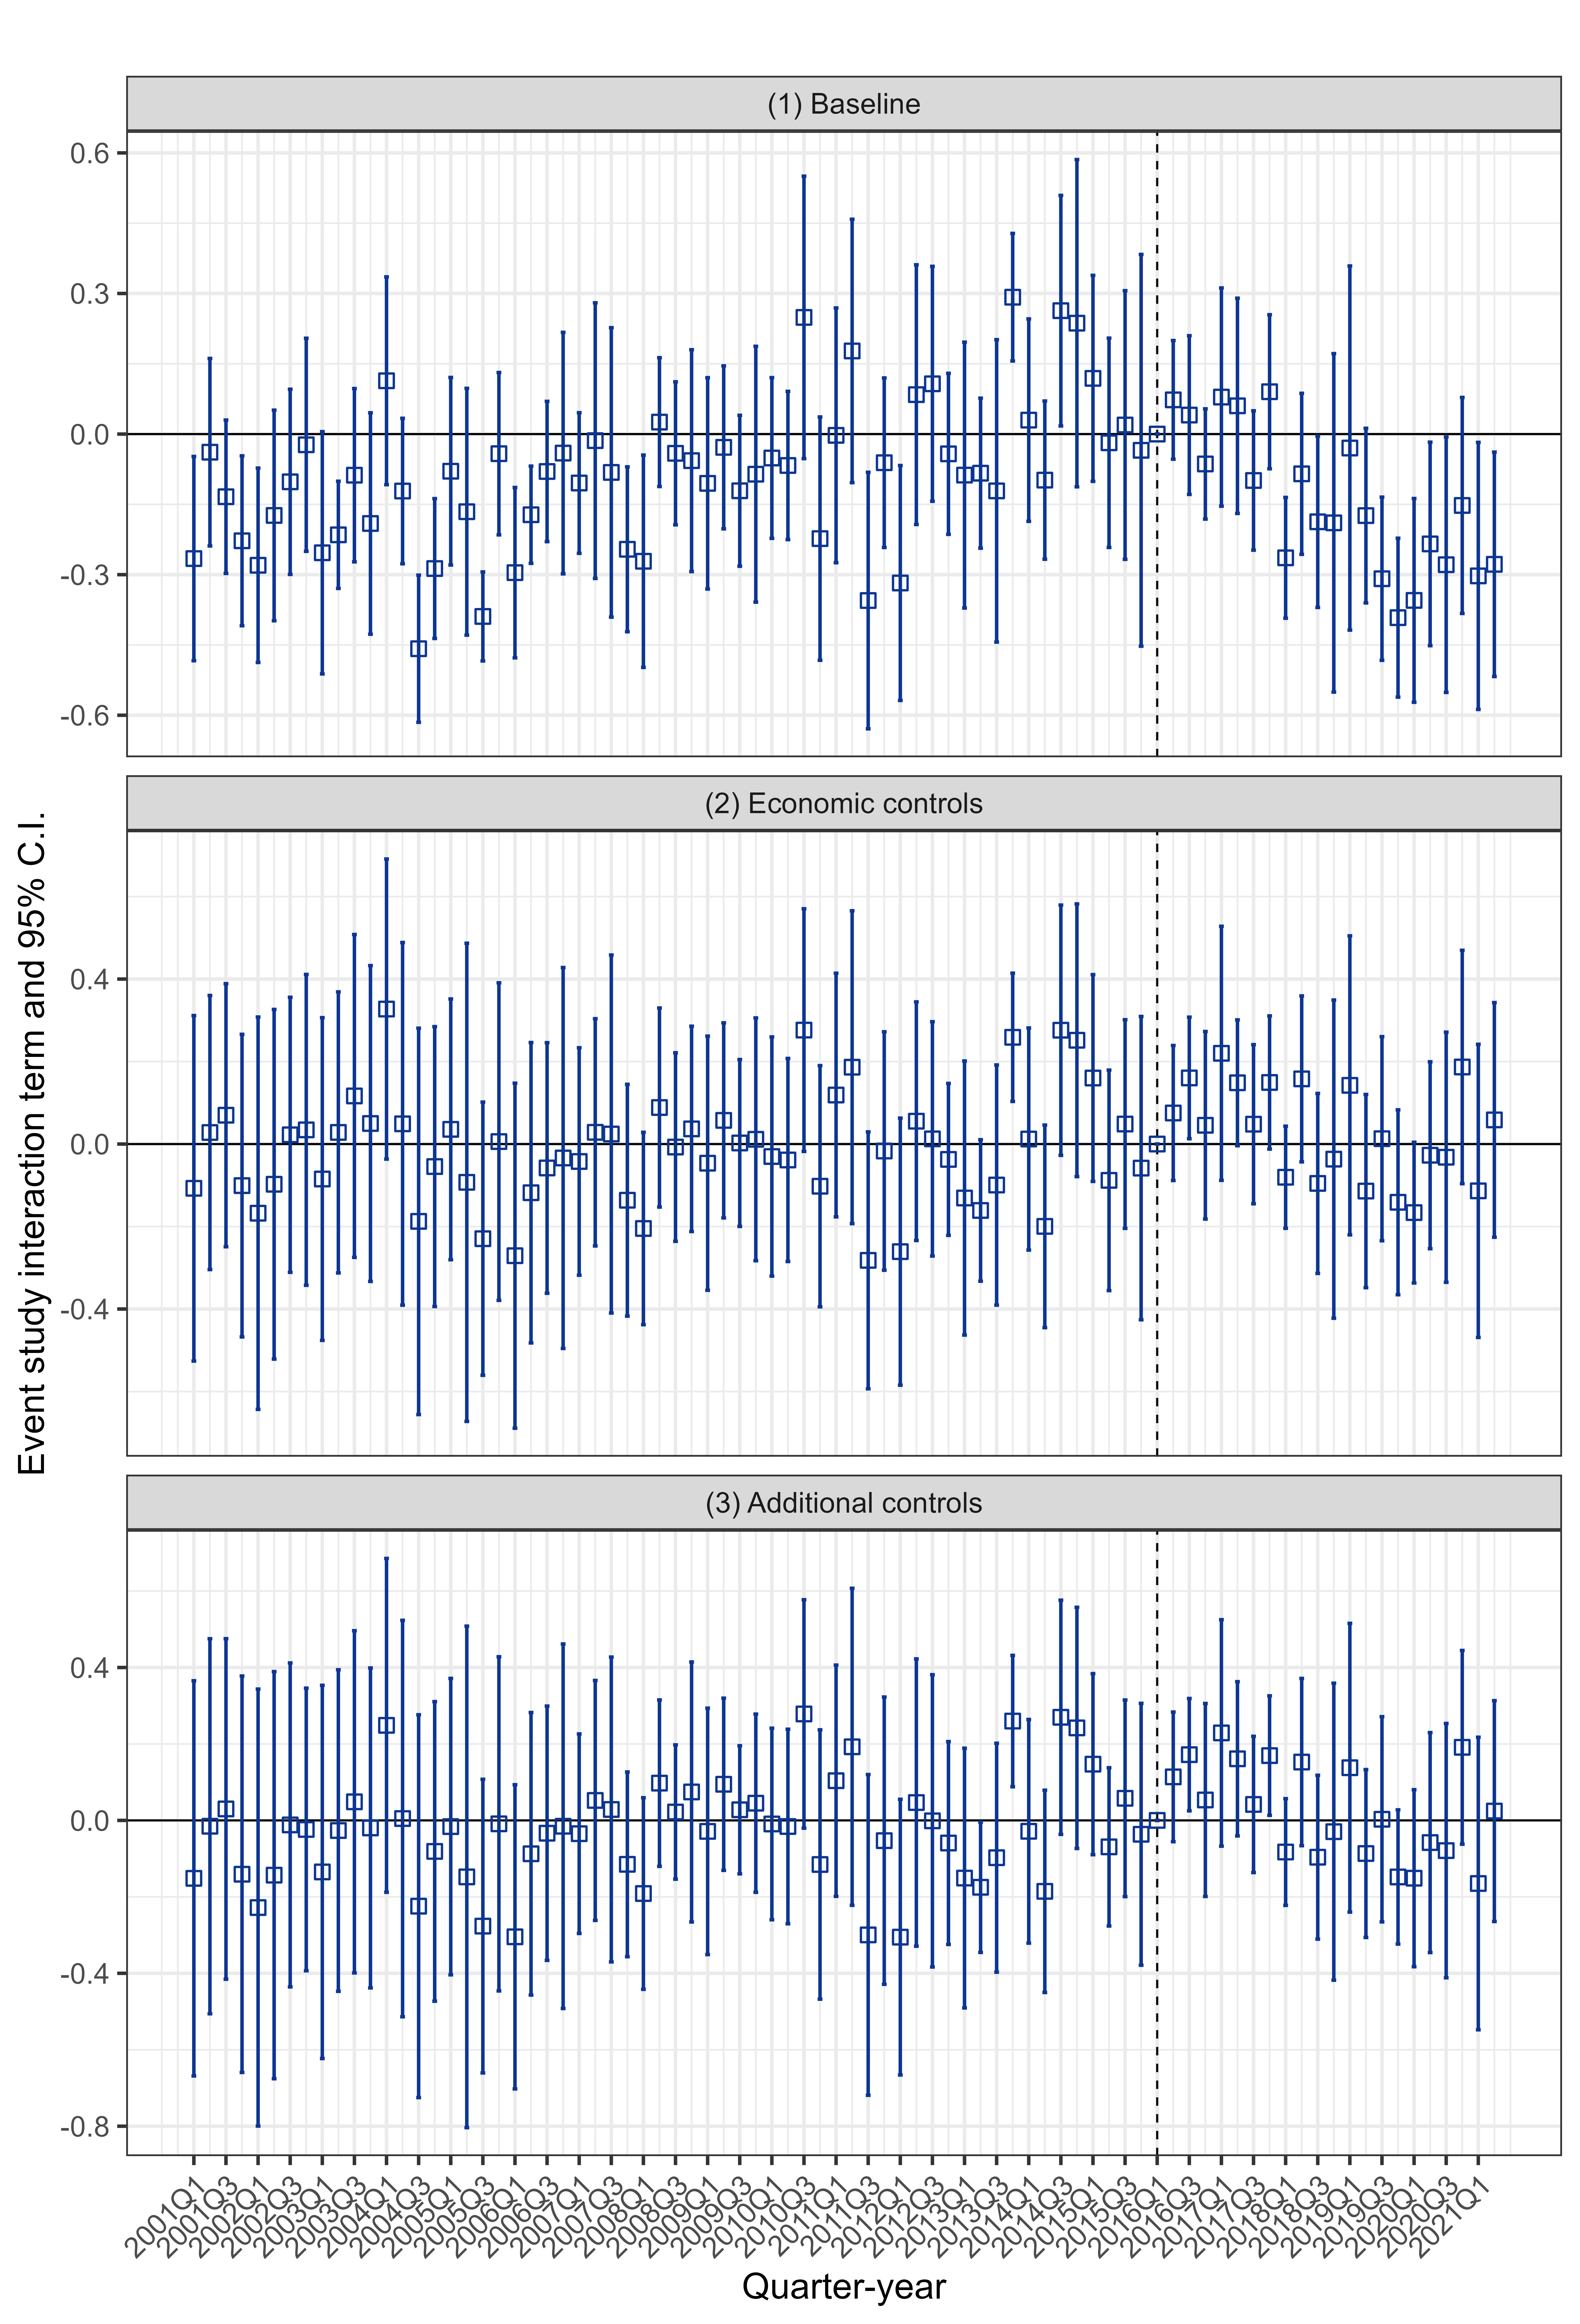
\includegraphics{\subfix{../../figures/event-studies/quarterly/patents_faceted.png}}
    \begin{minipage}{0.9\textwidth}
        \footnotesize
        \textit{Notes}: The figure shows the estimated coefficients of the interaction term between period and treatment binary variables in Equation \ref{eq:event_study} for each quarter. The points represent the point estimate, while the ribbons represent the 95\% confidence cluster-robust interval. The vertical line represents the start of the AITC intervention (first expense eligibility date) in April 2016, with the reference level being the quarter before the intervention. Baseline, economic, and additional controls specifications include the controls seen in specifications (1) through (3) in Table \ref{tab:dd_twfe_patents}. 
    \end{minipage}
\end{figure}

Regarding the effect of the policy itself, results point toward statistical insignificance of the policy effect. While there is a small positive effect in 2016Q4, it is unlikely that this is due to the policy, as the effect is not present in the following quarters. There is no evidence of a negative effect of the policy on patent applications, as preliminarily shown by the time series plot in Figure \ref{fig:quarterly_common_trends}.

\subsection{Patents by section}

In Table \ref{tab:dd_twfe_patents_by_section}, I present the results of the estimation of Equation \ref{eq:dd_model}, allowing for heterogeneity by IPC patent section and including the controls of Specification (3) in Table \ref{tab:dd_twfe_patents}. The results show that the AITC intervention had no statistically significant effect on most of the IPC sections, except sections A and E, corresponding to human necessities and fixed constructions. The effect on section A is positive and significant, while the effect on section E is negative and significant. These two effects are of similar magnitude (between |42.7|\% to |53.0|\%), suggesting an offseting effect of the policy. 
   
\begin{table}[h]
    \centering
    \label{tab:dd_twfe_patents_by_section}
\begin{threeparttable}
    \caption{Difference-in-differences results for quarterly patent applications by IPC section}
    
\begin{tabular}[t]{lcccccccc}
\toprule
  & (1) & (2) & (3) & (4) & (5) & (6) & (7) & (8)\\
\midrule
Treatment x Post & \num{0.427}*** & \num{0.366} & \num{0.066} & \num{0.235} & \num{-0.530}*** & \num{0.167} & \num{-0.083} & \num{0.209}\\
\textbf{} & \textbf{(\num{0.071})} & \textbf{(\num{0.195})} & \textbf{(\num{0.171})} & \textbf{(\num{0.132})} & \textbf{(\num{0.045})} & \textbf{(\num{0.106})} & \textbf{(\num{0.187})} & \textbf{(\num{0.135})}\\
\midrule
Patent section (IPC) & A & B & C & D & E & F & G & H\\
$N$ & \num{656} & \num{656} & \num{656} & \num{656} & \num{656} & \num{656} & \num{656} & \num{656}\\
Adj. $R^2$ & \num{0.913} & \num{0.911} & \num{0.879} & \num{0.353} & \num{0.914} & \num{0.875} & \num{0.910} & \num{0.908}\\
Adj. within $R^2$ & \num{0.111} & \num{0.056} & \num{0.082} & \num{0.033} & \num{0.061} & \num{0.021} & \num{0.060} & \num{0.063}\\
RMSE & \num{0.324} & \num{0.355} & \num{0.381} & \num{0.356} & \num{0.361} & \num{0.394} & \num{0.395} & \num{0.409}\\
\bottomrule
\end{tabular}
}
    \begin{tablenotes}
        \small
        \item \textit{Notes}: Sections of the IPC are A: Human Necessities, B: Performing Operations; Transporting, C: Chemistry; Metallurgy, D: Textiles; Paper, E: Fixed Constructions, F: Mechanical Engineering; G: Physics, H: Electricity. Patents with multiple sections are not included. 
        \item All specifications include controls in Specification (3) of Table \ref{tab:dd_twfe_patents}, not shown for brevity and fixed effects for provinces and quarters. Clustered standard errors at the province and quarter level shown in parentheses. ***$p<0.01$, **$p<0.05$, *$p<0.1$.
    \end{tablenotes}
\end{threeparttable}
\end{table}

Because I lose precision on the estimates due to the smaller sample size, I am underpowered to detect small effects on the other sections. The event study regressions in Figure provide additional insight into the effect of the policy on patent applications by IPC section. 
\end{document}

